% !TEX program = xelatex
\documentclass[UTF8,zihao=-4,oneside,openany]{ctexbook}

% Shared style for the combined handout.  Section files keep standalone
% preambles for now, while the master document uses this single definition.
\usepackage[a4paper,top=20mm,bottom=22mm,left=19mm,right=19mm,headheight=24pt]{geometry}
\usepackage[table]{xcolor}
\usepackage{amsmath,amssymb,mathtools,bm}
\usepackage{siunitx}
\usepackage{booktabs,tabularx,array,multicol}
\usepackage{enumitem}
\usepackage{tikz}
\usetikzlibrary{arrows.meta,positioning,calc,angles,quotes,patterns}
\usepackage[most]{tcolorbox}
\usepackage{fancyhdr}
\usepackage{hyperref}

\definecolor{Ink}{HTML}{202326}
\definecolor{DeepBlue}{HTML}{294E69}
\definecolor{Blue}{HTML}{47687D}
\definecolor{PaleBlue}{HTML}{F3F5F6}
\definecolor{Gold}{HTML}{6E777D}
\definecolor{PaleGold}{HTML}{F6F6F5}
\definecolor{Green}{HTML}{5B6D76}
\definecolor{PaleGreen}{HTML}{F3F5F6}
\definecolor{Alert}{HTML}{666B6F}
\definecolor{PaleAlert}{HTML}{F6F6F6}
\definecolor{RuleGray}{HTML}{D3D7DA}
\definecolor{TextGray}{HTML}{61686D}
\definecolor{SoftGray}{HTML}{F6F6F6}

\color{Ink}
\sisetup{
  per-mode=symbol,
  inter-unit-product=\ensuremath{{}\cdot{}},
  exponent-product=\times
}

\hypersetup{
  colorlinks=true,
  linkcolor=DeepBlue,
  urlcolor=Blue,
  pdfsubject={高中物理竞赛一轮资料重排讲义},
  pdfauthor={物理竞赛一轮资料编写组}
}

\setlength{\parindent}{2em}
\setlength{\parskip}{0.25em}
\setlist{nosep,leftmargin=2em}
\setcounter{secnumdepth}{3}
\setcounter{tocdepth}{2}
\numberwithin{equation}{section}
\counterwithin{table}{section}
\allowdisplaybreaks[2]
\emergencystretch=2em

\ctexset{
  chapter={
    format=\raggedright\LARGE\bfseries\color{Ink},
    titleformat=\LARGE\bfseries\color{Ink},
    beforeskip=0pt,
    afterskip=18pt
  },
  section={
    format=\Large\bfseries\color{DeepBlue},
    beforeskip=1.8ex,
    afterskip=1.0ex
  },
  subsection={
    format=\large\bfseries\color{Ink},
    beforeskip=1.5ex,
    afterskip=0.8ex
  },
  subsubsection={format=\normalsize\bfseries\color{Ink}}
}

\pagestyle{fancy}
\fancyhf{}
\fancyhead[L]{\small\color{TextGray}高中物理竞赛一轮讲义}
\fancyhead[R]{\small\color{TextGray}第一章\quad 数学与物理工具}
\fancyfoot[C]{\small\color{TextGray}\thepage}
\renewcommand{\headrulewidth}{0.4pt}
\renewcommand{\headrule}{\hbox to\headwidth{\color{RuleGray}\leaders\hrule height \headrulewidth\hfill}}

\newcommand{\dimens}[1]{\operatorname{dim}\!\left(#1\right)}
\newcommand{\dd}{\mathop{}\!\mathrm{d}}
\newcommand{\vect}[1]{\bm{#1}}
\newcommand{\uvec}[1]{\hat{\vect{#1}}}
\newcommand{\e}{\mathrm e}
\newcommand{\order}[1]{\mathcal O\!\left(#1\right)}
\DeclareMathOperator{\proj}{proj}
\newcommand{\examplesource}[1]{%
  \par{\small\color{TextGray}题源：#1}\par
}

\newtcolorbox{goalbox}{
  enhanced,breakable,
  colback=PaleBlue,colframe=Blue,
  boxrule=0.7pt,arc=2mm,
  title={本节目标},fonttitle=\bfseries,
  coltitle=DeepBlue,
  attach boxed title to top left={xshift=5mm,yshift=-2mm},
  boxed title style={colback=white,colframe=Blue,boxrule=0.7pt,arc=1.5mm}
}

\newtcolorbox{sourcebox}{
  enhanced,breakable,
  colback=SoftGray,colframe=RuleGray,
  boxrule=0.5pt,arc=0mm,
  title={题源说明},fonttitle=\bfseries,
  coltitle=Ink,colbacktitle=SoftGray,
  borderline west={1.2pt}{0pt}{TextGray}
}

\newtcolorbox[auto counter,number within=section]{examplebox}[2][]{
  enhanced,breakable,
  colback=white,colframe=RuleGray,
  boxrule=0.5pt,arc=0mm,
  title={例题~\thetcbcounter\quad #2},fonttitle=\bfseries,
  coltitle=Ink,colbacktitle=PaleBlue,
  borderline west={1.4pt}{0pt}{DeepBlue},
  #1
}

\newtcolorbox{methodbox}[1]{
  enhanced,breakable,
  colback=PaleBlue,colframe=RuleGray,
  boxrule=0.5pt,arc=0mm,
  title={方法：#1},fonttitle=\bfseries,
  coltitle=Ink,colbacktitle=PaleBlue,
  borderline west={1.2pt}{0pt}{DeepBlue}
}

\newtcolorbox{warningbox}[1]{
  enhanced,breakable,
  colback=SoftGray,colframe=RuleGray,
  boxrule=0.5pt,arc=0mm,
  title={易错提醒：#1},fonttitle=\bfseries,
  coltitle=Ink,colbacktitle=SoftGray,
  borderline west={1.2pt}{0pt}{TextGray}
}

\newtcolorbox{extensionbox}[1]{
  enhanced,breakable,
  colback=PaleGold,colframe=Gold,
  boxrule=0.5pt,arc=0mm,
  title={拓展：#1},fonttitle=\bfseries,
  coltitle=Ink,colbacktitle=PaleGold,
  borderline west={1.2pt}{0pt}{DeepBlue}
}

\newtcolorbox{summarybox}{
  enhanced,breakable,
  colback=PaleBlue,colframe=DeepBlue,
  boxrule=0.9pt,arc=1.5mm,
  title={本节小结},fonttitle=\bfseries,
  coltitle=white,colbacktitle=DeepBlue
}

\newtcolorbox{exercisebox}[1]{
  enhanced,breakable,
  colback=white,colframe=RuleGray,
  boxrule=0.7pt,arc=1.5mm,
  title={#1},fonttitle=\bfseries,
  coltitle=DeepBlue,colbacktitle=PaleBlue
}

\tikzset{
  vector/.style={-{Latex[length=2.5mm]},very thick,draw=DeepBlue},
  component/.style={-{Latex[length=2.2mm]},thick,draw=TextGray},
  axis/.style={-{Latex[length=2mm]},thin,draw=TextGray},
  guide/.style={densely dashed,draw=TextGray},
  curve/.style={very thick,draw=DeepBlue},
  tangent/.style={thick,draw=TextGray},
  secant/.style={thick,draw=DeepBlue}
}


\hypersetup{
  pdftitle={高中物理竞赛一轮讲义：第一章第二节 受力分析（含解答与解图）},
  pdfsubject={以学而思一轮资料为基础重新组织，并补写完整解答}
}

\fancyhead[R]{\small\color{TextGray}第一章\quad 静力学}
\renewcommand{\theequation}{\thechapter.\arabic{equation}}

\newtcolorbox{origexamplebox}[1]{
  enhanced,
  colback=white,colframe=RuleGray,
  boxrule=0.5pt,arc=0mm,
  title={#1},fonttitle=\bfseries,
  coltitle=Ink,colbacktitle=PaleBlue,
  borderline west={1.4pt}{0pt}{DeepBlue}
}

\newenvironment{xesolution}{%
  \par\smallskip
  \begingroup\small
  \setlength{\abovedisplayskip}{4pt plus 2pt minus 1pt}%
  \setlength{\belowdisplayskip}{4pt plus 2pt minus 1pt}%
  \setlength{\abovedisplayshortskip}{3pt plus 1pt}%
  \setlength{\belowdisplayshortskip}{3pt plus 1pt minus 1pt}%
  \noindent{\bfseries\color{DeepBlue}解答}\quad
}{%
  \par\endgroup\medskip
}

\begin{document}

\pagenumbering{arabic}
\setcounter{page}{1}
\setcounter{chapter}{1}
\setcounter{section}{1}

\section{受力分析}
\setcounter{equation}{7}

当一个物体受多个力作用时，需要给定所有力的大小、方向和作用点才能够完全了解它的
受力情况。对质点，多个力可合成为一个力；对刚体，若各力的作用线通过同一点，称为共点力，
也可用通过该点的合力代替。其合力为几个力的矢量和：
\begin{equation}
  \vec{F}=\sum_i\vec{F}_i.
\end{equation}
一般刚体上的非共点力还可能产生力偶；此时仅知道矢量和不足以说明转动效果，必须同时
考虑合力矩。例如两个等大反向、作用线不重合的力，合力为零，却仍能使物体转动。

当在坐标系中分析受力时，将一个给定的力向着坐标轴的方向分解对处理问题也是有帮助
的。这里采用沿正交坐标轴的投影分解；沿某个正轴的分量是有符号的数，不能把它与非负的力的大小混为一谈。

若所选单位轴为 $\hat{\boldsymbol e}$，则力沿该轴的\textbf{有符号分量}可统一写成
\[
  F_e=\vec F\cdot\hat{\boldsymbol e}=F\cos\theta.
\]
当投影方向与正轴相反时，$F_e<0$。这个负号已包含方向信息，不应再人为补一个负号。
相应的分矢量是 $F_e\hat{\boldsymbol e}$，它的大小为 $|F_e|$。若使用非正交方向作斜分解，
则需联立矢量方程，不能把每个分力都直接写成余弦投影。

\begin{origexamplebox}{例 1.8}
如图所示，有五个力 $\vec{F}_1,\vec{F}_2,\vec{F}_3,\vec{F}_4,\vec{F}_5$ 作用于一点 $O$，
构成一个正六边形的两邻边和三条对角线。设 $F_3=\SI{10}{\newton}$，试求这五个力的合力。

\begin{center}
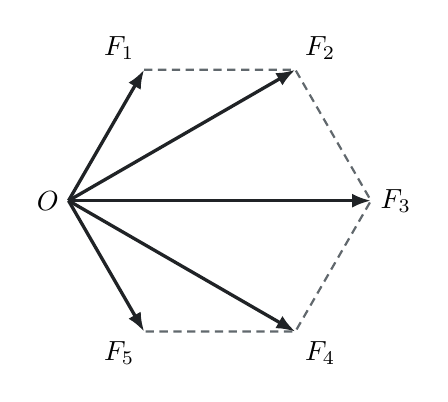
\begin{tikzpicture}[scale=0.64]
  \coordinate (O)  at (-3,0);
  \coordinate (F1) at (-1.5,2.598);
  \coordinate (F2) at (1.5,2.598);
  \coordinate (F3) at (3,0);
  \coordinate (F4) at (1.5,-2.598);
  \coordinate (F5) at (-1.5,-2.598);

  \draw[guide,thick] (F1)--(F2)--(F3)--(F4)--(F5);
  \foreach \P in {F1,F2,F3,F4,F5}{
    \draw[-{Latex[length=2.4mm]},very thick,draw=Ink] (O)--(\P);
  }

  \node[left] at (O) {$O$};
  \node[above left] at (F1) {$F_1$};
  \node[above right] at (F2) {$F_2$};
  \node[right] at (F3) {$F_3$};
  \node[below right] at (F4) {$F_4$};
  \node[below left] at (F5) {$F_5$};
\end{tikzpicture}
\end{center}
\end{origexamplebox}

\begin{xesolution}
图中各力的大小就是相应矢量的几何长度。沿 $F_3$ 方向取 $x$ 轴，正六边形的边长设为 $s$，则
\[
  F_3=2s.
\]
关于 $x$ 轴对称的两对力的竖直分量相互抵消；水平分量分别为
\[
  \vec F_1+\vec F_5=s\,\hat{\boldsymbol i}
  =\frac12\vec F_3,
\]
\[
  \vec F_2+\vec F_4=3s\,\hat{\boldsymbol i}
  =\frac32\vec F_3.
\]
因而
\[
  \vec F_{\rm sum}
  =\left(\frac12+\frac32+1\right)\vec F_3
  =3\vec F_3.
\]
已知 $F_3=\SI{10}{\newton}$，所以
\[
  \boxed{F_{\rm sum}=\SI{30}{\newton}},
\]
方向与 $\vec F_3$ 相同。
\end{xesolution}

找出力学系统中每个物体受力的大小、方向和作用点的过程称为受力分析，一般来说在
静力学中主要考虑上面提到过的几种典型的受力。除了特别的假设，地面附近所有物体都受
重力，发生形变的弹性物体有弹力作用，相互接触的表面之间有可能有压力，当有压力并且
有相对运动或相对运动趋势时还可能有摩擦力。除此之外，在有的问题中还可能出现大气压
力、浮力等其它种类的力，做受力分析的时候要把所有重要的因素全部考虑方可。

虽然力的效果在物理上是一致的，但不同的力也有细微的区别。在做受力分析时，可以
将力分为两大类，一类称做主动力，例如重力、弹簧弹力等。这些力的共同特点就是它们可
由系统的状态直接确定，只要知道了物体的质量、弹簧的弹性系数和形变量以后就可以确定
其大小和方向。另一类称约束力或被动力，例如支持力、两个物体连接处的作用力等，它们
无法直接确定，是由主动力和限制物体运动约束的性质共同决定。

从建立未知量的角度看，主动力通常可由相互作用律直接写出，例如近地重力 $mg$ 和线性
弹簧力 $-kx$；约束力则通常需要与平衡方程或运动方程联立求出。这一划分是建模工具，
不是对力的微观来源进行分类。

\begin{origexamplebox}{例 1.9}
\begin{minipage}[c]{0.62\linewidth}
均匀长棒一端搁在地面上，另一端用细线系在天花板上，如图所示，若细线竖直，
试分析棒的受力情况。
\end{minipage}\hfill
\begin{minipage}[c]{0.34\linewidth}
\centering

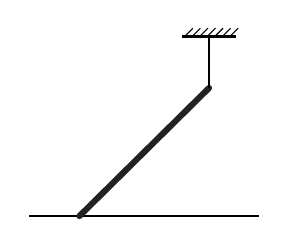
\begin{tikzpicture}[scale=0.48]
  \draw[thick] (-3.1,-1.7)--(3.0,-1.7);
  % Model the long rod by its centre line, so its lower endpoint has
  % single-point contact with the floor rather than face contact.
  \draw[draw=Ink,line width=2.2pt,line cap=round]
    (-1.76,-1.70)--(1.67,1.69);
  \draw[thick] (1.67,1.69)--(1.67,3.05);
  \draw[thick] (0.95,3.05)--(2.39,3.05);
  \foreach \x in {1.02,1.22,...,2.32}{
    \draw[thin] (\x,3.05)--++(0.22,0.22);
  }
\end{tikzpicture}
\end{minipage}
\end{origexamplebox}

\begin{xesolution}
隔离木棒。对图示的非竖直木棒，需要考虑中点处的重力 $mg$、上端细线的竖直张力 $T$、
下端地面的法向力 $N$ 和水平摩擦力未知量 $f$。图中灰色虚线只表示 $f$ 的预设正方向，
并不表示摩擦力一定非零。

\begin{center}
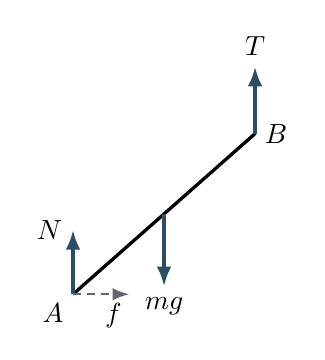
\begin{tikzpicture}[scale=0.68]
  \coordinate (A) at (-1.8,-1.2); \coordinate (B) at (1.6,1.8); \coordinate (C) at ($(A)!0.5!(B)$);
  \draw[very thick] (A)--(B);
  \draw[vector] (B)--++(0,1.25) node[above]{$T$};
  \draw[vector] (C)--++(0,-1.35) node[below]{$mg$};
  \draw[vector] (A)--++(0,1.2) node[left]{$N$};
  \draw[-{Latex[length=2.1mm]},thick,draw=TextGray,densely dashed]
    (A)--++(1.05,0) node[pos=0.72,below=3pt,inner sep=0pt]{$f$};
  \node[below left] at (A) {$A$}; \node[right] at (B) {$B$};
\end{tikzpicture}
\end{center}

水平方向只有 $f$，由平衡条件立即得
\[
  \boxed{f=0}.
\]
力矩衡量力使物体绕参考点转动的作用，其大小为力乘参考点到作用线的垂直距离（力臂）。
取逆时针为正，平衡时各力矩的代数和为零。设木棒与水平面夹角为 $\theta$\ ($\cos\theta\ne0$)，
对下端 $A$ 取矩：$N$ 和 $f$ 的作用线都通过 $A$，力臂为零；$T$ 和 $mg$ 均竖直，
它们的力臂分别为水平距离 $L\cos\theta$ 和 $(L/2)\cos\theta$，转动趋势相反。因此
\[
  T(L\cos\theta)-mg\left(\frac L2\cos\theta\right)=0,
\]
所以
\[
  \boxed{T=\frac{mg}{2}},\qquad
  \boxed{N=mg-T=\frac{mg}{2}}.
\]
灰色虚线仅标明 $f$ 的预设正方向；求得 $f=0$ 说明接触并不意味着摩擦力非零。
若木棒恰好竖直，三个竖直力共线，力矩方程不能分别确定 $T$ 与 $N$，只能得到 $T+N=mg$。
\end{xesolution}

\end{document}
